\documentclass[11pt]{article}

\usepackage{custom}

\title{605.744: Information Retrieval \\ Programming Assignment \#5: Near Duplicate Detection}
\author{Sabbir Ahmed}
\date{\today}

\begin{document}
\maketitle
\tableofcontents
\clearpage
\newpage

\section{Introduction}
This paper describes detecting near-duplications (plagiarism) within documents in datasets of various sample sizes.

\section{Technical Background}
All of the source code is in Python 3.10. The program is split into several modules and follows an object oriented structure.

% .
% ├── ir/
% │   ├── __init__.py
% │   ├── files.py
% │   ├── minhash.py
% │   └── text.py
% ├── models/
% ├── outputs/
% └── run.py

\begin{figure}[!ht]
  \centering
  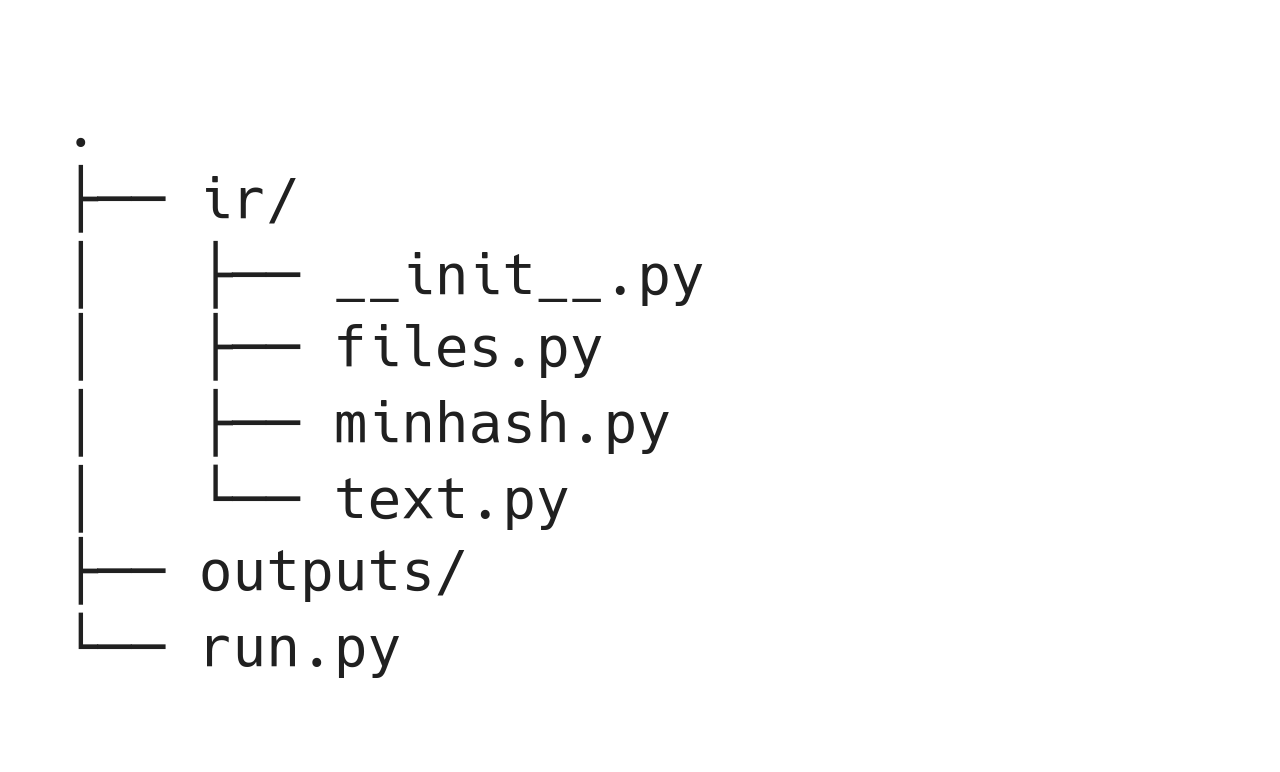
\includegraphics[trim={0 3cm 15cm 3cm},clip,scale=0.3]{statics/dirtree.png}
  \caption{Directory Hierarchy of Assignment 5}
\end{figure}

The source code for all of the files are attached in Appendix \ref{appendix:src}.

The total number of non-empty lines of code for the program totals to under 285.

\begin{figure}[!ht]
  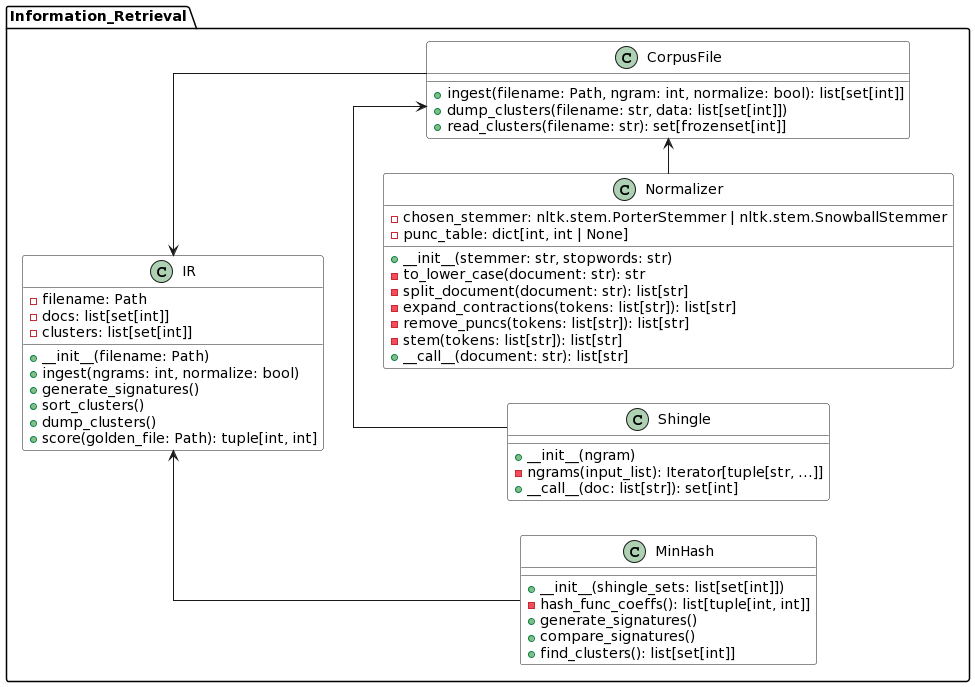
\includegraphics[scale=0.45]{statics/uml.png}
  \centering
  \caption{UML of Information Retrieval}
\end{figure}

\subsection{Classes}
Some classes from Assignment 3 were used in this project:
\begin{itemize}
  \item the driver script \texttt{run.py} was modified with the relevant flags
  \item the \texttt{files.CorpusFile} class was modified to process TSV files and read and write clusters to disk
  \item the \texttt{text.Normalizer} class was used to normalize documents into lists of stemmed words
\end{itemize}

\subsection{\texttt{text.Shingle}}

\subsection{\texttt{minhash.MinHash}}
The hash functions \cite{leskovec_rajaraman_ullman_2022}

\subsection{External Libraries}
The following external libraries were used to implement portions of the assignment:
\begin{itemize}
  \item Natural Language Toolkit (NLTK) \cite{bird2009natural}
  \item NetworkX \cite{SciPyProceedings_11}
\end{itemize}

\section{Scoring}

\begin{simptable}
  {Distribution of \textit{Assessment} in the training dataset}
  {dist_train}
  {| c | c | c | c |}
  \textbf{N-Gram} & \textbf{Normalized} & \textbf{$G-O$} & \textbf{$O-G$}
  \\ \hline
  \textbf{1} & True & 2 & 1
  \\ \hline
  \textbf{1} & False & 2 & 2
  \\ \hline
  \textbf{2} & True & 1 & 2
  \\ \hline
  \textbf{2} & False & 3 & 2
  \\ \hline
  \textbf{3} & True & 2 & 4
  \\ \hline
  \textbf{3} & False & 2 & 4
  \\ \hline
  \textbf{4} & True & 3 & 6
  \\ \hline
  \textbf{4} & False & 3 & 6
  \\ \hline
  \textbf{5} & True & 3 & 6
  \\ \hline
  \textbf{5} & False & 4 & 9
  \\ \hline
  \textbf{6} & True & 10 & 12
  \\ \hline
  \textbf{6} & False & 10 & 12
  \\ \hline
\end{simptable}

\addcontentsline{toc}{section}{References}
\bibliographystyle{ieeetr}
\bibliography{refs}

\appendix
\addcontentsline{toc}{section}{Appendix}

\section{Source Code} \label{appendix:src}

\inputpython{../ir/\_\_init\_\_.py}{ir/\_\_init\_\_.py}
\inputpython{../ir/files.py}{ir/files.py}
\inputpython{../ir/minhash.py}{ir/minhash.py}
\inputpython{../ir/text.py}{ir/text.py}

\inputpython{../run.py}{run.py}

\end{document}
